%!TEX root=thesis.tex

\section{Reinforcement Learning}

% TODO think about what I want to put in here vs what I want to put into the methods section. Just put high-level introduction, and possible relevant to ham engineering?

\begin{quote}
    Reinforcement learning is learning what to do--how to map situations to actions--so as to maximize a numerical reward signal. \cite{sutton2018reinforcement}
\end{quote}
Reinforcement learning  (RL) has been applied to a variety of different problems, including interacting with physical environments such as balancing a pole \cite{lillicrap2015continuous} or playing games such as chess or Go \cite{Silver1140}. A significant attraction of RL is its generality: in most cases no prior knowledge of the problem is assumed. As a result, any problem that can be formulated as a Markov decision process (MDP) can be approached with RL.

% potential application to Ham engineering
Hamiltonian engineering fits into the RL paradigm by considering discrete time steps. Changes to the control Hamiltonian parameters are actions applied to the environment, the propagator is the state, and the overlap or fidelity of the propagator with the target propagator is the reward.  Each of these are developed in more detail below.

% \subsection{Important RL Concepts}

In the language of RL, an \emph{agent} is responsible for performing \emph{actions} on the \emph{environment} to maximize a \emph{reward signal} (or reward). The agent can see the \emph{state} of the environment which informs what actions to take. See figure~\ref{fig:RL} for a diagram of the agent-environment interactions. In turn, the agent's actions may affect the environment state. The agent must then balance exploration of the environment by choosing a variety of actions and exploitation of its prior knowledge to maximize rewards.
For a more detailed description of the RL framework, see \cite{sutton2018reinforcement}.

\begin{figure}
    \centering
    % \scalebox{.5}{
    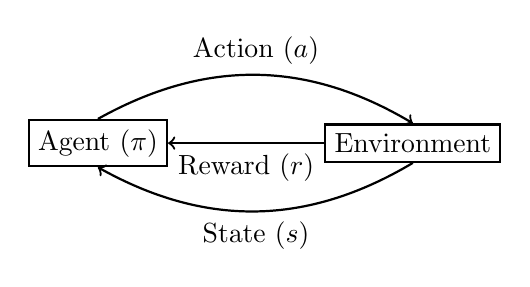
\begin{tikzpicture}[->, thick]
         %nodes
         \node[draw] at (-2,0) (agent) {Agent ($\pi$)}; % : S \to \mathcal{P}(A)
         \node[draw] at (2,0) (env) {Environment};
         \path
             (agent.north) edge[bend left=30] node[above] {Action ($a$)} (env.north)
             (env.south) edge[bend left=30] node[below] {State ($s$)} (agent.south)
             (env.west) edge node[below] {Reward ($r$)} (agent.east);
    \end{tikzpicture}
    % }
    \caption{The general reinforcement learning paradigm.}
    \label{fig:RL}
\end{figure}

The agent decides what actions to perform via a policy function $\pi$, which maps from a state $s \in S$ to either a probability distribution over the action space $\mathcal{P}(A)$ (a ``stochastic policy'') or simply a particular action $a \in A$ (a ``deterministic policy''). Policy functions are typically implemented as neural networks which are then usually optimized using gradient-based methods.

There are a few other common functions used in RL. The \emph{return} at time step $t$ is defined as
\begin{equation}\label{eq:return}
    G_t \defeq \sum_{k=t}^T \gamma^{k-t} R_k, \quad \gamma \in [0,1)
\end{equation}
or the total discounted rewards until the end of the episode at time step $T$. The \emph{state-value function} is the expected return from a particular state while following a policy $\pi$
\begin{equation}\label{eq:state_value}
    v_\pi(s) \defeq \E[G_t | S_t = s]
\end{equation}
Finally, the \emph{action-value function} is the expected return from taking an action $a$ in state $s$, then after following policy $\pi$
\begin{equation}\label{eq:action_value}
    q_\pi(s, a) \defeq \E[G_t | S_t = s, A_t = a]
\end{equation}

\subsection{Action space}

The action space can generally be discrete (there are finitely many actions that can be performed) or continuous  (infinitely many actions). The size of the action space determines the type of RL algorithm that can be used. In discrete action spaces, the policy can be stochastic and learn a probability distribution over every action. In continuous action spaces, where it's impractical to learn an arbitrary probability distribution over all actions, the policy can either be stochastic and learn parameters of a general probability distribution (such as a multivariate Gaussian) or deterministic and return the action.

For Hamiltonian engineering, the size of the action space depends on the number of allowed control Hamiltonians. As an example, in many pulse sequences developed using average Hamiltonian theory, the control Hamiltonians are restricted to $\pi/2$-pulses at consistent time intervals, which is better suited to a discrete action space. In contrast, techniques such as GRAPE
\cite{Khaneja-2005}
allow the control Hamiltonian amplitudes to vary continuously.

Both discrete and continuous action spaces were tested, and the results of each are shared below in the sections for each corresponding RL algorithm.

\subsection{Reward schemes}

The goal of Hamiltonian engineering is to control the system so that its time-evolution appears to be under some effective Hamiltonian. The reward signal should then be larger when the actual evolution is ``close'' to the target evolution. One measure of ``closeness'' is the fidelity function for two unitary operators
\begin{equation} % TODO make sure this is right
    F(U_\text{actual}, U_\text{target}) = \left| \frac{\Tr{
        U_\text{actual}^\dagger U_\text{target}
    }}{\Tr{\identity}} \right|
\end{equation}
The fidelity approaches 1 as the unitaries get closer, and approaches 0 as the unitaries get further apart. However, a tenfold improvement in performance doesn't correspond to a tenfold increase in fidelity (take for instance a fidelity of 0.9 compared to 0.99). A suitable reward function is then calculated by
\begin{equation}
    R = -\log(1-F(U_\text{actual}, U_\text{target}) + \epsilon)
\end{equation}
where $\epsilon>0$ ensures the reward isn't infinite.

There is also the decision of \emph{when} to give rewards to the agent. A reward can be given at every time step during the episode (``dense rewards'') or only at certain time steps such as the end of the episode (``sparse rewards'').
Dense rewards make sense when the fidelity matters at every time step, such as implementing a target unitary in the shortest amount of time possible.
% TODO does ^ make sense? May need to explain more...
Sparse rewards make sense when the fidelity only matters at certain points in time, such as in stroboscopic measurements and pulse sequences.

\subsection{State space and state representation}

The state space is the set of all possible states of the system. A possible approach would be to encode the state as the density matrix or propagator at the current time step. However, the density matrix and propagator grow exponentially as the system size increases, and the complete characterization of the quantum system is unrealistic for any experimental application.

An alternative state representation is the sequence of past actions applied to the system.  This representation generally requires less memory and computation, and may also be better suited to more robust control.

\subsection{Algorithm Examples}

There are many RL algorithms that have been developed, tailored to different characteristics of the RL problem. The relevant characteristics include
\begin{description}
    \item[Model] An agent in a \emph{model-free} RL algorithm learns a policy directly from observations of the environment. An agent in a \emph{model-based} RL algorithm instead uses observations to model the environment, then uses that model to learn a policy.
    \item[Policy] An \emph{on-policy} algorithm improves the policy that is used to interact with the environment. An \emph{off-policy} algorithm has separate policies for improvement and environment interaction.
    \item[Action space] As mentioned before, an action space can be \emph{discrete} (finitely many actions) or \emph{continuous} (infinitely many actions).
\end{description}
In addition to the above characteristics, there are general classes of RL algorithms, such as temporal-difference learning policy gradient methods. More information on RL can be found in \cite{sutton2018reinforcement}.

% TODO put in a diagram showing model-free, model, online, offline, etc....

The AlphaZero algorithm was used as the primary RL algorithm in this work, and a more complete description of the algorithm can be found in the Methods section. The other algorithms listed below were explored as potential options for Hamiltonian engineering, but ultimately were not as effective as AlphaZero.

\subsubsection{Q-learning and DQN}

Q-learning is a model-free, off-policy, TD control algorithm applicable to discrete action spaces \cite{watkins1989learning}. As the name suggests, the action-value function $Q(s,a)$ is learned from experiences with the environment according to the following update rule
\begin{equation}\label{eq:Q_learning_update}
    Q(S_t, A_t) \leftarrow Q(S_t, A_t) +
        \alpha \left[ R_{t+1} + \gamma \max_a Q(S_{t+1}, a) - Q(S_t, A_t) \right]
\end{equation}
To encourage exploration of the state and action spaces, the agent typically follows an $\epsilon$-greedy policy (with probability $1-\epsilon$ perform the action that maximizes $Q$, otherwise perform a random action), which makes this algorithm \emph{off-policy}.

If the state and action spaces are small, then it's feasible for all the $Q$-values to be stored in memory. In general, though, the action-value function is approximated using a neural network, and the parameters are updated to minimize the loss given by \ref{eq:Q_learning_update}. This approach is called ``deep Q-network'' or DQN \cite{mnih2013playing}. DQN is suitable for large state spaces (as demonstrated through Atari games in \cite{mnih2013playing}), but still requires the action space to be discrete.

% TODO include DDPG??
% \subsubsection{DDPG}
%
% ``Deep deterministic policy gradient'' (DDPG) extends the idea of deep reinforcement learning in DQNs to continuous action spaces \cite{lillicrap2015continuous}. As with DQN, DDPG is a model-free, off-policy algorithm, but uses an actor-critic framework that separates the policy and the value function estimators. In addition, the policy is deterministic, so it returns a single action instead of a distribution over actions. As the agent interacts with the environment, the experiences are recorded in a \emph{replay buffer} on which the actor and critic are trained. The critic is updated by minimizing the sampled value estimate errors,
% % TODO include update equation?
% % \begin{align}\label{eq:DDPG_critic_update}
% %     L = \frac{1}{N} \sum_i (y_i - Q(S_i, A_i | \theta^Q))^2 \\
% %     y_i = R_i + \gamma Q'(S_{i+1}, \mu'(S_{i+1}|\theta^{\mu'}) |\theta^{Q'})
% % \end{align}
% and the actor is updated using the sampled policy gradient%
% % TODO include?
% % \begin{equation}
% %     \nabla_{\theta^\mu} J \approx \frac{1}{N} \sum_i
% %     \nabla_a Q(s, a | theta^Q)|_{s=s_i, a=\mu(s_i)}
% %     \nabla_{\theta^\mu} \mu(s|\theta^\mu)|_{s_i}
% % \end{equation}
% .

\subsubsection{AlphaZero}


AlphaZero is a model-based, off-policy, actor-critic algorithm that was originally developed to play Chess, Shogi, and Go \cite{Silver1140}. There are two major components to the algorithm: self-play and training. Because AlphaZero is a model-based algorithm, the agent is able to consider the state space without necessarily interacting with the environment. The agent plays many episodes against itself, using a neural network to estimate a policy $\pi(s)$ and a value function $v_\pi(s)$. During self-play, the agent rolls out many possible state-action trajectories, chooses an action that maximizes the expected reward, and collects data on the state, which actions it considered, and the final reward at the end of the episode. The collected data in turn is used to train the policy and value neural networks $\{ \pi, v_\pi \}$.

% TODO more here, also include diagram?

\subsubsection{PPO}

Proximal-policy optimization (PPO) is a model-free, on-policy actor-critic algorithm that tried to improve data efficiency and robustness compared to existing algorithms (such as DQN or other policy gradient methods).
\cite{schulman2017proximal}.
In contrast with other policy gradient methods, the PPO objective function is clipped according to a hyperparameter $\epsilon$.
\begin{equation}\label{eq:ppo_loss}
    % eq 7 in PPO paper
    L(\theta) = \E_t \left[\min(
        r_t(\theta)\hat{A}_t,
        \text{clip}(r_t(\theta), 1-\epsilon, 1+\epsilon) \hat{A}_t
    )\right]
\end{equation}
where
$r_t(\theta) = \frac{\pi_\theta(a_t|s_t)}{\pi_{\theta'}(a_t|s_t)}$ is the probability ratio of actions under the new and old policies, and $\hat{A}_t$ is an estimator of the \emph{advantage function} at time $t$. By clipping the objective, the gradient updates are non-zero only for a region close to the previous policy, thus preventing policy changes that are too large.
PPO has been applied successfully to both continuous and discrete action spaces%
% TODO check above, I think that's right but not sure...
.

\subsubsection{ERL}

Evolutionary reinforcement learning (ERL) is a model-free, off-policy hybrid algorithm that uses both actor-critic policy gradient and evolutionary algorithm methods \cite{khadka2018evolutionguided}. ERL addresses problems found in many  gradient-based RL algorithms, including temporal credit assignment (associating actions to rewards that may be separated by many time steps), exploration of the state and action spaces, and policy convergence sensitivity to hyperparameters. To do so, ERL maintains a population of actors with individual policies that interact with the environment. The population's experiences are recorded in a shared replay buffer, and a separate actor/critic pair learn from the replay buffer using policy gradient (such as DDPG or DQN). Periodically, the policy gradient-based actor is copied into the population, and evolutionary algorithms are used to iterate a new ``generation'' of actors (by preferentially selecting high-performing actors). By using both gradient-based and gradient-free methods, ERL attempts to achieve both efficiency and policy diversity, making it a candidate for a variety of RL problems.
